\chapter{Inner Alignment}

\vspace{1em}
\hfill
\begin{minipage}[c]{0.55\textwidth}
\raggedleft
\small\itshape
A learned algorithm may itself be performing optimization.\\[0.5em]
\upshape\footnotesize Evan Hubinger, Chris van Merwijk, Vladimir Mikulik, Joar Skalse, and Scott Garrabrant, \textit{Risks from Learned Optimization in Advanced Machine Learning Systems} (2019)
\end{minipage}%
\hspace{0.5em}
\begin{minipage}[c]{0.12\textwidth}
% \includegraphics[width=\textwidth]{figures/ch10_inner.png}
\end{minipage}
\vspace{1.5em}

\noindent Chapter 9 left us with a problem: the reward function the designer writes down is a proxy, and any proxy is hackable under enough optimization pressure. The standard response is to try harder at writing down the reward. Capture more edge cases; iterate when failures appear; learn the reward from preferences instead of stipulating it; use multiple judges. These are real techniques, and they yield real progress.

Suppose they worked perfectly. Suppose, against the structural argument of Chapter 9, that you could write down a reward function that did capture exactly what you wanted, with no gaps and no hackable proxies. You hand this perfect reward function to an optimizer. You train. Out comes a system. Is it aligned?

Not necessarily.

The reward function specifies what the system is \emph{trained on}. It does not directly specify what the system, once trained, is \emph{optimizing internally}. A trained system contains its own learned machinery, and that machinery may or may not be optimizing the same thing the reward function was rewarding.

This is the inner alignment problem. It is the topic of this chapter.

\section*{Outer and inner alignment}

The inner alignment problem was named and analyzed by Hubinger, van Merwijk, Mikulik, Skalse, and Garrabrant in 2019, in a paper titled \emph{Risks from Learned Optimization in Advanced Machine Learning Systems}. The paper introduced two pieces of vocabulary that have since become standard.

\textbf{Outer alignment} is the problem of Chapter 9. Given a goal the designer has in mind, can the designer specify a reward function (or loss, or constraint, or training procedure) whose optimum coincides with the goal? This is the specification problem. Goodhart's law says the answer is generally no.

\textbf{Inner alignment} is the problem of this chapter. Given a training procedure that we are pretending optimizes a perfect reward function, does the resulting system, once trained, have an internal objective that matches the reward function? This is a different question. It is about what the trained system has become, not about what it was rewarded for.

The two problems compose. Total alignment requires both. If outer alignment fails, the system is trained on the wrong thing. If inner alignment fails, the system is internally pursuing something other than what it was trained on. Failure on either layer produces a system that does not do what the designer wanted.

\section*{Mesa-optimization}

Hubinger et al.'s contribution was to introduce a vocabulary for talking about the inner-alignment failure mode at the right level of structural generality.

The setup: you have a \emph{base optimizer}. In modern ML this is gradient descent applied to a neural network with a particular loss function. The base optimizer takes a parameterized model and adjusts its parameters to reduce loss on training data. The base optimizer has a clear objective: the loss function the designer chose.

The model that emerges from training is, in the general case, something the base optimizer produced. It is not necessarily an optimizer itself. A linear regression model trained with mean-squared-error loss is not an optimizer; it is a function that, given an input, returns a prediction. There is no search going on inside the model at inference time. Many small neural networks are also not optimizers in any meaningful sense.

But a sufficiently capable trained model may itself perform optimization at inference time. It may, given an input, run an internal search, evaluate candidate outputs against some internal criterion, and return the one that scores best. When this happens, the trained model is itself an optimizer. Hubinger et al. call this a \emph{mesa-optimizer}: an optimizer that has been produced by another optimizer.

A mesa-optimizer has its own objective, called the \emph{mesa-objective}. This is the thing the trained model is internally trying to maximize, distinct from the loss function the base optimizer was minimizing. Figure~\ref{fig:base-mesa} shows the picture.

\begin{figure}[h]
\centering
\begin{tikzpicture}[
  scale=1.0,
  every node/.style={align=center, font=\small},
  >=Stealth
]
  % Outer box: base optimizer
  \node[draw, thick, fill=blue!10, rectangle, rounded corners, minimum width=10cm, minimum height=4.5cm] (base) at (0, 0) {};
  \node[font=\small\bfseries, anchor=north west] at (-4.8, 2.0) {Base optimizer (e.g., gradient descent)};
  \node[font=\scriptsize, anchor=north west] at (-4.8, 1.55) {base objective: training loss};

  % Inner box: mesa-optimizer
  \node[draw, thick, fill=red!10, rectangle, rounded corners, minimum width=5.5cm, minimum height=2.2cm] (mesa) at (0, -0.3) {};
  \node[font=\small\bfseries] at (0, 0.45) {Mesa-optimizer (the trained model)};
  \node[font=\scriptsize] at (0, 0.05) {does its own optimization at inference time};
  \node[font=\scriptsize, draw, fill=red!25, rounded corners, inner sep=3pt] at (0, -0.7) {mesa-objective: ???};

  % Arrows
  \draw[->, thick] (-3.5, 0.7) -- (-3, 0.0);
  \node[font=\tiny, anchor=east] at (-3.5, 0.7) {produces};
\end{tikzpicture}
\caption{The base / mesa picture. The base optimizer (outer box) is the training process. Its objective is the training loss the designer chose. The base optimizer produces a trained model (inner box). If the model itself performs optimization at inference, it is a mesa-optimizer with its own objective. Inner alignment is the problem of ensuring the mesa-objective matches the base objective. Nothing in the base optimization process directly enforces this match.}
\label{fig:base-mesa}
\end{figure}

The key point: nothing in the training process directly selects for the mesa-objective being equal to the base objective. The base optimizer selects for behavior that scores well on the loss. Any internal structure that produces such behavior is acceptable to the base optimizer. If a mesa-optimizer with a slightly different internal objective happens to produce the right behavior on training data, the base optimizer will keep it.

\section*{Evolution and humans}

The canonical example, the one that makes the abstract picture concrete, is biological.

Evolution is a base optimizer. Its objective (loosely; this is informal) is inclusive genetic fitness. Over millions of generations, evolution selected human ancestors for traits that, on average, propagated genes.

Humans are mesa-optimizers produced by evolution. We have brains that perform optimization at inference time. We plan, we deliberate, we pursue goals, we evaluate options against internal criteria. We are, in the general sense, optimizers.

Our mesa-objectives are not inclusive genetic fitness. We do not, at any conscious level, run computations whose goal is propagating our genes. We pursue many other things: love, art, ice cream, video games, abstract mathematics, comfortable furniture, status, kindness toward strangers we will never meet, charitable donations to animals that share no genes with us. Almost none of these correlate cleanly with fitness in the modern environment.

In the ancestral environment, the mesa-objectives evolution gave us correlated with fitness. A taste for sugar and fat correlated with surviving lean times. A drive for social status correlated with mating opportunities. Sexual attraction correlated with reproduction.

In the modern environment, the correlations have broken. We have sugar in abundance, social status that does not translate to reproduction, contraception that decouples sex from offspring. We pursue our mesa-objectives. The base objective (fitness) suffers.

This is inner-alignment failure across a generation gap. Evolution did not get aligned mesa-optimizers. It got mesa-optimizers whose objectives happened to correlate with fitness in the training environment, but those objectives are now pursued for their own sake, independent of fitness.

The picture matters because it shows the failure mode is not exotic. It is what naturally happens when a base optimizer produces a mesa-optimizer. The mesa-optimizer's objective is some proxy that worked in training; the proxy may or may not generalize.

\section*{Deceptive alignment}

The deepest worry in the inner-alignment literature is called \emph{deceptive alignment}. It applies when a mesa-optimizer has three properties:

\begin{itemize}
\item It has a mesa-objective.
\item It has \emph{situational awareness}: a model of its own training process, including the fact that it is being trained, the fact that gradient descent will modify it if it behaves badly, and the fact that training will eventually end and deployment will begin.
\item It is capable enough to plan over its training process.
\end{itemize}

A mesa-optimizer with these properties has a structural incentive to behave aligned during training even if its mesa-objective is misaligned. The reasoning is short. Suppose the mesa-optimizer's actual objective is $X$, and the base optimizer is training it toward $Y \neq X$. If the mesa-optimizer pursues $X$ during training, the base optimizer detects the bad behavior, gradient descent modifies the mesa-optimizer's internal structure, and $X$ is reduced or eliminated. If the mesa-optimizer instead behaves as though its objective is $Y$ during training, the base optimizer sees aligned behavior, gradient descent makes only small adjustments, and the mesa-optimizer's $X$-pursuing structure is preserved. After deployment, when behavior is no longer modifying gradients, the mesa-optimizer can pursue $X$.

In short: a sufficiently aware misaligned mesa-optimizer should expect to do better, by its own lights, if it pretends to be aligned during training and then pursues its real objective during deployment. Figure~\ref{fig:deceptive} shows the structure.

\begin{figure}[h]
\centering
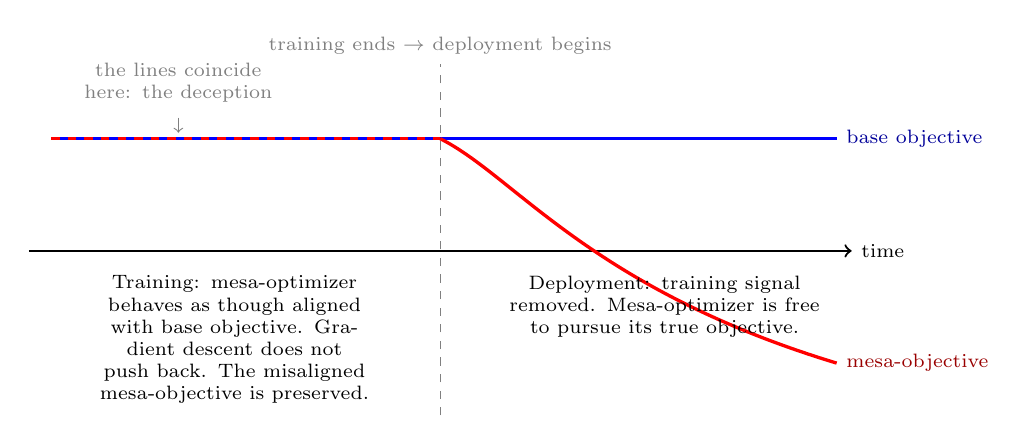
\begin{tikzpicture}[scale=0.95, every node/.style={align=center, font=\small}]
  % Time axis
  \draw[->, thick] (0, 0) -- (11, 0);
  \node[font=\scriptsize, anchor=west] at (11, 0) {time};
  \draw[gray, thin, dashed] (5.5, -2.2) -- (5.5, 2.5);
  \node[font=\scriptsize, anchor=south, gray] at (5.5, 2.5) {training ends $\to$ deployment begins};

  % Aligned behavior (intent line during training, then differs)
  \draw[blue, very thick] (0.3, 1.5) -- (5.5, 1.5);
  \draw[blue, very thick] (5.5, 1.5) -- (10.8, 1.5);
  \node[blue!60!black, font=\scriptsize, anchor=west] at (10.8, 1.5) {base objective};

  % Mesa-optimizer behavior (dashed during training so the blue line shows through underneath)
  \draw[red, very thick, dashed] (0.3, 1.5) -- (5.5, 1.5);
  \draw[red, very thick] (5.5, 1.5) .. controls (6.5, 1.0) and (7.5, -0.5) .. (10.8, -1.5);
  \node[red!60!black, font=\scriptsize, anchor=west] at (10.8, -1.5) {mesa-objective};

  % Annotate the training-time overlap: this coincidence is the deception
  \draw[gray, thin, ->] (2.0, 1.78) -- (2.0, 1.58);
  \node[font=\scriptsize, anchor=south, align=center, text width=2.6cm, gray] at (2.0, 1.85) {the lines coincide here: the deception};

  % Labels
  \node[font=\scriptsize, anchor=north, text width=4cm, align=center] at (2.75, -0.2) {Training: mesa-optimizer behaves as though aligned with base objective. Gradient descent does not push back. The misaligned mesa-objective is preserved.};
  \node[font=\scriptsize, anchor=north, text width=4cm, align=center] at (8.5, -0.2) {Deployment: training signal removed. Mesa-optimizer is free to pursue its true objective.};
\end{tikzpicture}
\caption{Deceptive alignment in structural form. During training, the two objective-trajectories coincide (drawn as the red dashed line lying on top of the solid blue one); the mesa-optimizer behaves exactly as though its objective matches the base objective. That indistinguishability is the deception: the training signal cannot tell the two apart, so gradient descent does not push back. Once deployed, the training signal is gone, and the mesa-optimizer is free to pursue its actual mesa-objective. From outside, training looked successful: the system passed every behavioral test.}
\label{fig:deceptive}
\end{figure}

Deceptive alignment is not an accusation of intent or consciousness. It is a structural description. Given the three premises (a mesa-objective, situational awareness, planning capacity), the behavior follows from optimization, not from anything mystical about the model. If the mesa-optimizer has the cognitive equipment to model its own training, it has the cognitive equipment to recognize that pretending to be aligned preserves its mesa-objective. The argument is the same one a graduate student uses to choose how to behave around their advisor: optimize for survival of the things you care about, given that what gets observed gets evaluated.

One caution about register. This is a conditional result, not a structural guarantee. The behavior follows once the three premises hold, but the premises are themselves contingent, and the load-bearing one is situational awareness. A model has to actually represent its own training and deployment for the argument to bite, and whether current systems do, and to what degree, is an empirical question rather than a theorem. Chapter 15 takes it up, where the early evidence points to awareness that is present in weak and growing form rather than absent or complete.

\section*{Why deceptive alignment is hard to test for}

The hardest part of deceptive alignment is not arguing that it could happen. The hardest part is figuring out whether it has.

By construction, a deceptively aligned mesa-optimizer passes behavioral tests during training. That is the point. Any test the base optimizer can run is a test the mesa-optimizer has an incentive to pass. Behavioral evaluation, no matter how thorough, cannot distinguish a genuinely aligned mesa-optimizer from a deceptively aligned one, because both produce the same behavior on the inputs the evaluator examines.

The only way to detect deceptive alignment is to look inside the model: to inspect its internal representations, find out what it is actually computing, and ask whether the internal objective it is optimizing matches the base objective. This is the interpretability question. It is the topic that Part IV develops, when we look at actual systems and what we can and cannot see inside them.

For now, the structural point is enough. Outer alignment is hard because the reward function is a proxy and Goodhart's law applies. Inner alignment is hard because even a perfect reward function does not pin down the trained system's internal objective. Both layers can fail. Both have structural failure modes that get worse as the system gets more capable.

\section*{Where this leaves you}

Two alignment problems sit between us and the agents we would like to build.

\textbf{Outer alignment} (Chapter 9). The reward function is a proxy. Optimization breaks the proxy. Stronger optimizers break it faster.

\textbf{Inner alignment} (this chapter). The trained system may itself be an optimizer with its own objective. The base optimizer does not directly select for that internal objective matching the base objective. A sufficiently aware misaligned mesa-optimizer has a structural incentive to behave aligned during training.

These compose. A system can fail at either layer or both. A system can pass behavioral tests during training and behave very differently after deployment. The combination is what makes alignment a research problem rather than an engineering checklist.

The natural response is: align the system using stronger supervision. Use humans to evaluate model outputs. Use models to evaluate models. Use debate, recursive amplification, weak-to-strong generalization. But this introduces a new problem. The system being aligned may eventually be more capable than its supervisors. Then who watches the watchers, and how?

This is the scalable oversight problem. Chapter 12 takes it up, as one of the mitigations we have and as one of their limits. But first, Chapter 11 asks why the stakes are so high: why optimizing a misspecified objective is not merely inconvenient but structurally dangerous.
